% IEEE ISCAS Format Paper
% Fed-RIS: Federated Phase Optimization for Tiled Reconfigurable Intelligent Surfaces via On-Chip Learning
\documentclass[conference]{IEEEtran}

\usepackage{amsmath,amssymb,amsfonts}
\usepackage{algorithmic}
\usepackage{graphicx}
\usepackage{textcomp}
\usepackage{xcolor}
\usepackage{cite}
\usepackage{booktabs}
\usepackage{multirow}
\usepackage{url}
\usepackage{bm}
\usepackage{siunitx}
\usepackage{subfig}

% Path to figures
\graphicspath{{results/figures/}{results/link_level/}}

\begin{document}

\title{Fed-RIS: Distributed Phase Optimization for Reconfigurable Intelligent Surfaces via On-Chip Federated Learning}

\author{\IEEEauthorblockN{Anonymous Author(s)}
\IEEEauthorblockA{Affiliation}
}

\maketitle

%% ===================================================================
%% ABSTRACT
%% ===================================================================
\begin{abstract}
Reconfigurable intelligent surfaces (RIS) require real-time channel-state information (CSI) to optimize their reflection phases, yet gathering raw CSI from every element to a central controller is bandwidth-intensive and privacy-invasive. We propose \textbf{Fed-RIS}, a federated learning framework that distributes phase optimization across the physical tiles of a single RIS. A 1024-element surface is partitioned into a $4\!\times\!4$ grid of 16 tiles, each containing $8\!\times\!8=64$ phase-controllable elements. Every tile trains a shared Graph Attention Network (GAT) phase predictor on its local CSI slice and exchanges only INT8 model deltas over an on-chip Network-on-Chip (NoC) interconnect---raw CSI never leaves the tile. We evaluate Fed-RIS against six baselines on identical 28\,GHz mmWave channel realizations with 30\,dB direct-path blockage. Fed-RIS recovers \textbf{36.7\,dB} of link budget over the blocked direct path, sits within \textbf{1.3\,dB} of the perfect-CSI MRC oracle bound, and degrades only \textbf{3.2\,dB} under severe CSI error ($\epsilon\!=\!1$) compared to 5.1\,dB for model-based solvers. Hardware impairments (phase quantization, jitter) are incorporated in-the-loop with measured penalties validated against classical theoretical bounds.
\end{abstract}

\begin{IEEEkeywords}
Reconfigurable intelligent surface, federated learning, graph attention network, network-on-chip, mmWave, phase optimization.
\end{IEEEkeywords}

%% ===================================================================
%% I. INTRODUCTION
%% ===================================================================
\section{Introduction}
\label{sec:intro}

Reconfigurable intelligent surfaces (RIS) have emerged as a transformative technology for beyond-5G wireless communications~\cite{wu2020joint, direnzo2020}. By controlling the reflection phase of each passive element, an RIS can constructively combine scattered paths and overcome severe blockage in millimeter-wave (mmWave) channels~\cite{rappaport2019}. The theoretical coherent array gain scales as $O(N^2)$ with the number of elements $N$~\cite{wu2020discrete}, making large surfaces highly attractive.

However, scaling RIS to thousands of elements introduces critical challenges. Conventional optimization approaches---alternating optimization (AO)~\cite{wu2020joint}, successive convex approximation (SCA)~\cite{guo2020}, ADMM~\cite{yu2020admm}, and semidefinite relaxation (SDR)~\cite{luo2010}---require full instantaneous CSI at a central controller and perform iterative solves per coherence block ($1.9$--$22$\,ms). Centralized deep learning (DL)~\cite{huang2020drl} amortizes inference to a single forward pass but still demands that raw CSI from every element be pooled at a central node.

We introduce \textbf{Fed-RIS}, which addresses these limitations through three key ideas:

\begin{enumerate}
\item \textbf{Surface-decomposed federation.} The RIS is physically partitioned into tiles, each acting as an independent federated learning (FL) client. Unlike conventional FL across user devices~\cite{mcmahan2017}, tiles share a coherent physical output---their phase contributions are summed electromagnetically. Non-IID data arises naturally from spatial geometry, not synthetic partitioning.

\item \textbf{Link-quality training objective.} Rather than regressing to precomputed MRC phase labels under MSE loss, the model directly optimizes a differentiable weighted sum-rate normalized by the genie-optimal rate, yielding gradients that reflect the true objective of coherent combining.

\item \textbf{On-chip aggregation with hardware fidelity.} Model deltas are exchanged via a modeled NoC (2D Torus, RingAllReduce protocol) with INT8 quantization. Phase quantization, jitter, and imperfect CSI are applied before scoring, with measured penalties validated against classical bounds.
\end{enumerate}

To the best of our knowledge, Fed-RIS is the first framework to federate phase optimization across the tiles of a single metasurface, model the on-chip communication cost with physical routing and energy accounting, and evaluate link-level communication metrics (BER, outage, spectral efficiency) across seven schemes on identical channel realizations.

%% ===================================================================
%% II. SYSTEM MODEL
%% ===================================================================
\section{System Architecture}
\label{sec:system}

\subsection{Propagation Model}

We consider a 28\,GHz mmWave link where a single-antenna base station (BS) at transmit power $P_\text{tx}=30$\,dBm communicates with a user through an RIS comprising $N=1024$ elements arranged in a $4\times4$ grid of 16 tiles, each containing $8\times8=64$ elements. The direct BS--user path suffers 30\,dB excess blockage loss~\cite{rappaport2019} with noise floor $\sigma^2=-90$\,dBm. The effective scalar channel is:
\begin{equation}
h_\text{eff} = h_\text{direct} + \sum_{t=1}^{T}\sum_{n=1}^{N_t} h_{\text{casc},t,n}\, e^{j\theta_{t,n}},
\label{eq:heff}
\end{equation}
where $h_\text{direct}$ is the attenuated direct channel, $h_{\text{casc},t,n} = h_{\text{ris-user},t,n} \cdot h_{\text{bs-ris},t,n}$ is the cascaded channel through element $n$ of tile~$t$, and $\theta_{t,n}$ is the controlled reflection phase. Channels follow a spatially correlated Rician model ($K\!=\!10$\,dB, $\rho\!=\!0.7$, 5 NLoS paths) with close-in path-loss exponents of 2.5 (RIS hops) and 3.5 (direct link), and per-element aperture gain $G_e = 4\pi A/\lambda^2$.

\subsection{On-Tile Federated Learning}

Each tile~$t$ acts as an FL client. From pilot-based channel estimates, tile~$t$ extracts its local cascaded coefficients as input features (real and imaginary parts, with per-block RMS normalization) and trains a shared 3-layer GAT phase predictor $f_{\bm{w}}: \hat{\bm{h}}_t \rightarrow \bm{\theta}_t$ using a differentiable sum-rate loss:
\begin{equation}
\mathcal{L} = 1 - \frac{\sum_u w_u \log_2\!\left(1 + \text{SINR}_u\right)}{R_\text{genie}},
\label{eq:loss}
\end{equation}
where $R_\text{genie}$ is the genie-optimal rate obtained by maximal-ratio combining (MRC) with perfect CSI. The global direct-path phase $\angle h_\text{direct}$ is factored out as sample-level metadata and added back at application time, preventing it from swamping per-element structure.

The GAT architecture constructs a 4-nearest-neighbor grid graph over the $8\times8$ tile elements with 8 attention heads, 256-dimensional hidden layers, and per-element cascade projections ($2U \rightarrow d$) to produce sample-specific node features. The output head predicts $(\cos\theta_n, \sin\theta_n)$ pairs to avoid the $0/2\pi$ wrap-around discontinuity.

\subsection{Network-on-Chip Aggregation}

After $E\!=\!3$ local epochs per tile, INT8 model weight deltas (1~byte/parameter, ${\sim}316$K parameters) are exchanged over a 2D Torus NoC at 10\,Gb/s using bandwidth-optimal RingAllReduce~\cite{patarasuk2009}. The server aggregates via FedAvg~\cite{mcmahan2017} across $R\!=\!20$ rounds. Raw CSI never traverses the interconnect. The system architecture is illustrated in Fig.~\ref{fig:arch}.

\begin{figure*}[t]
\centering
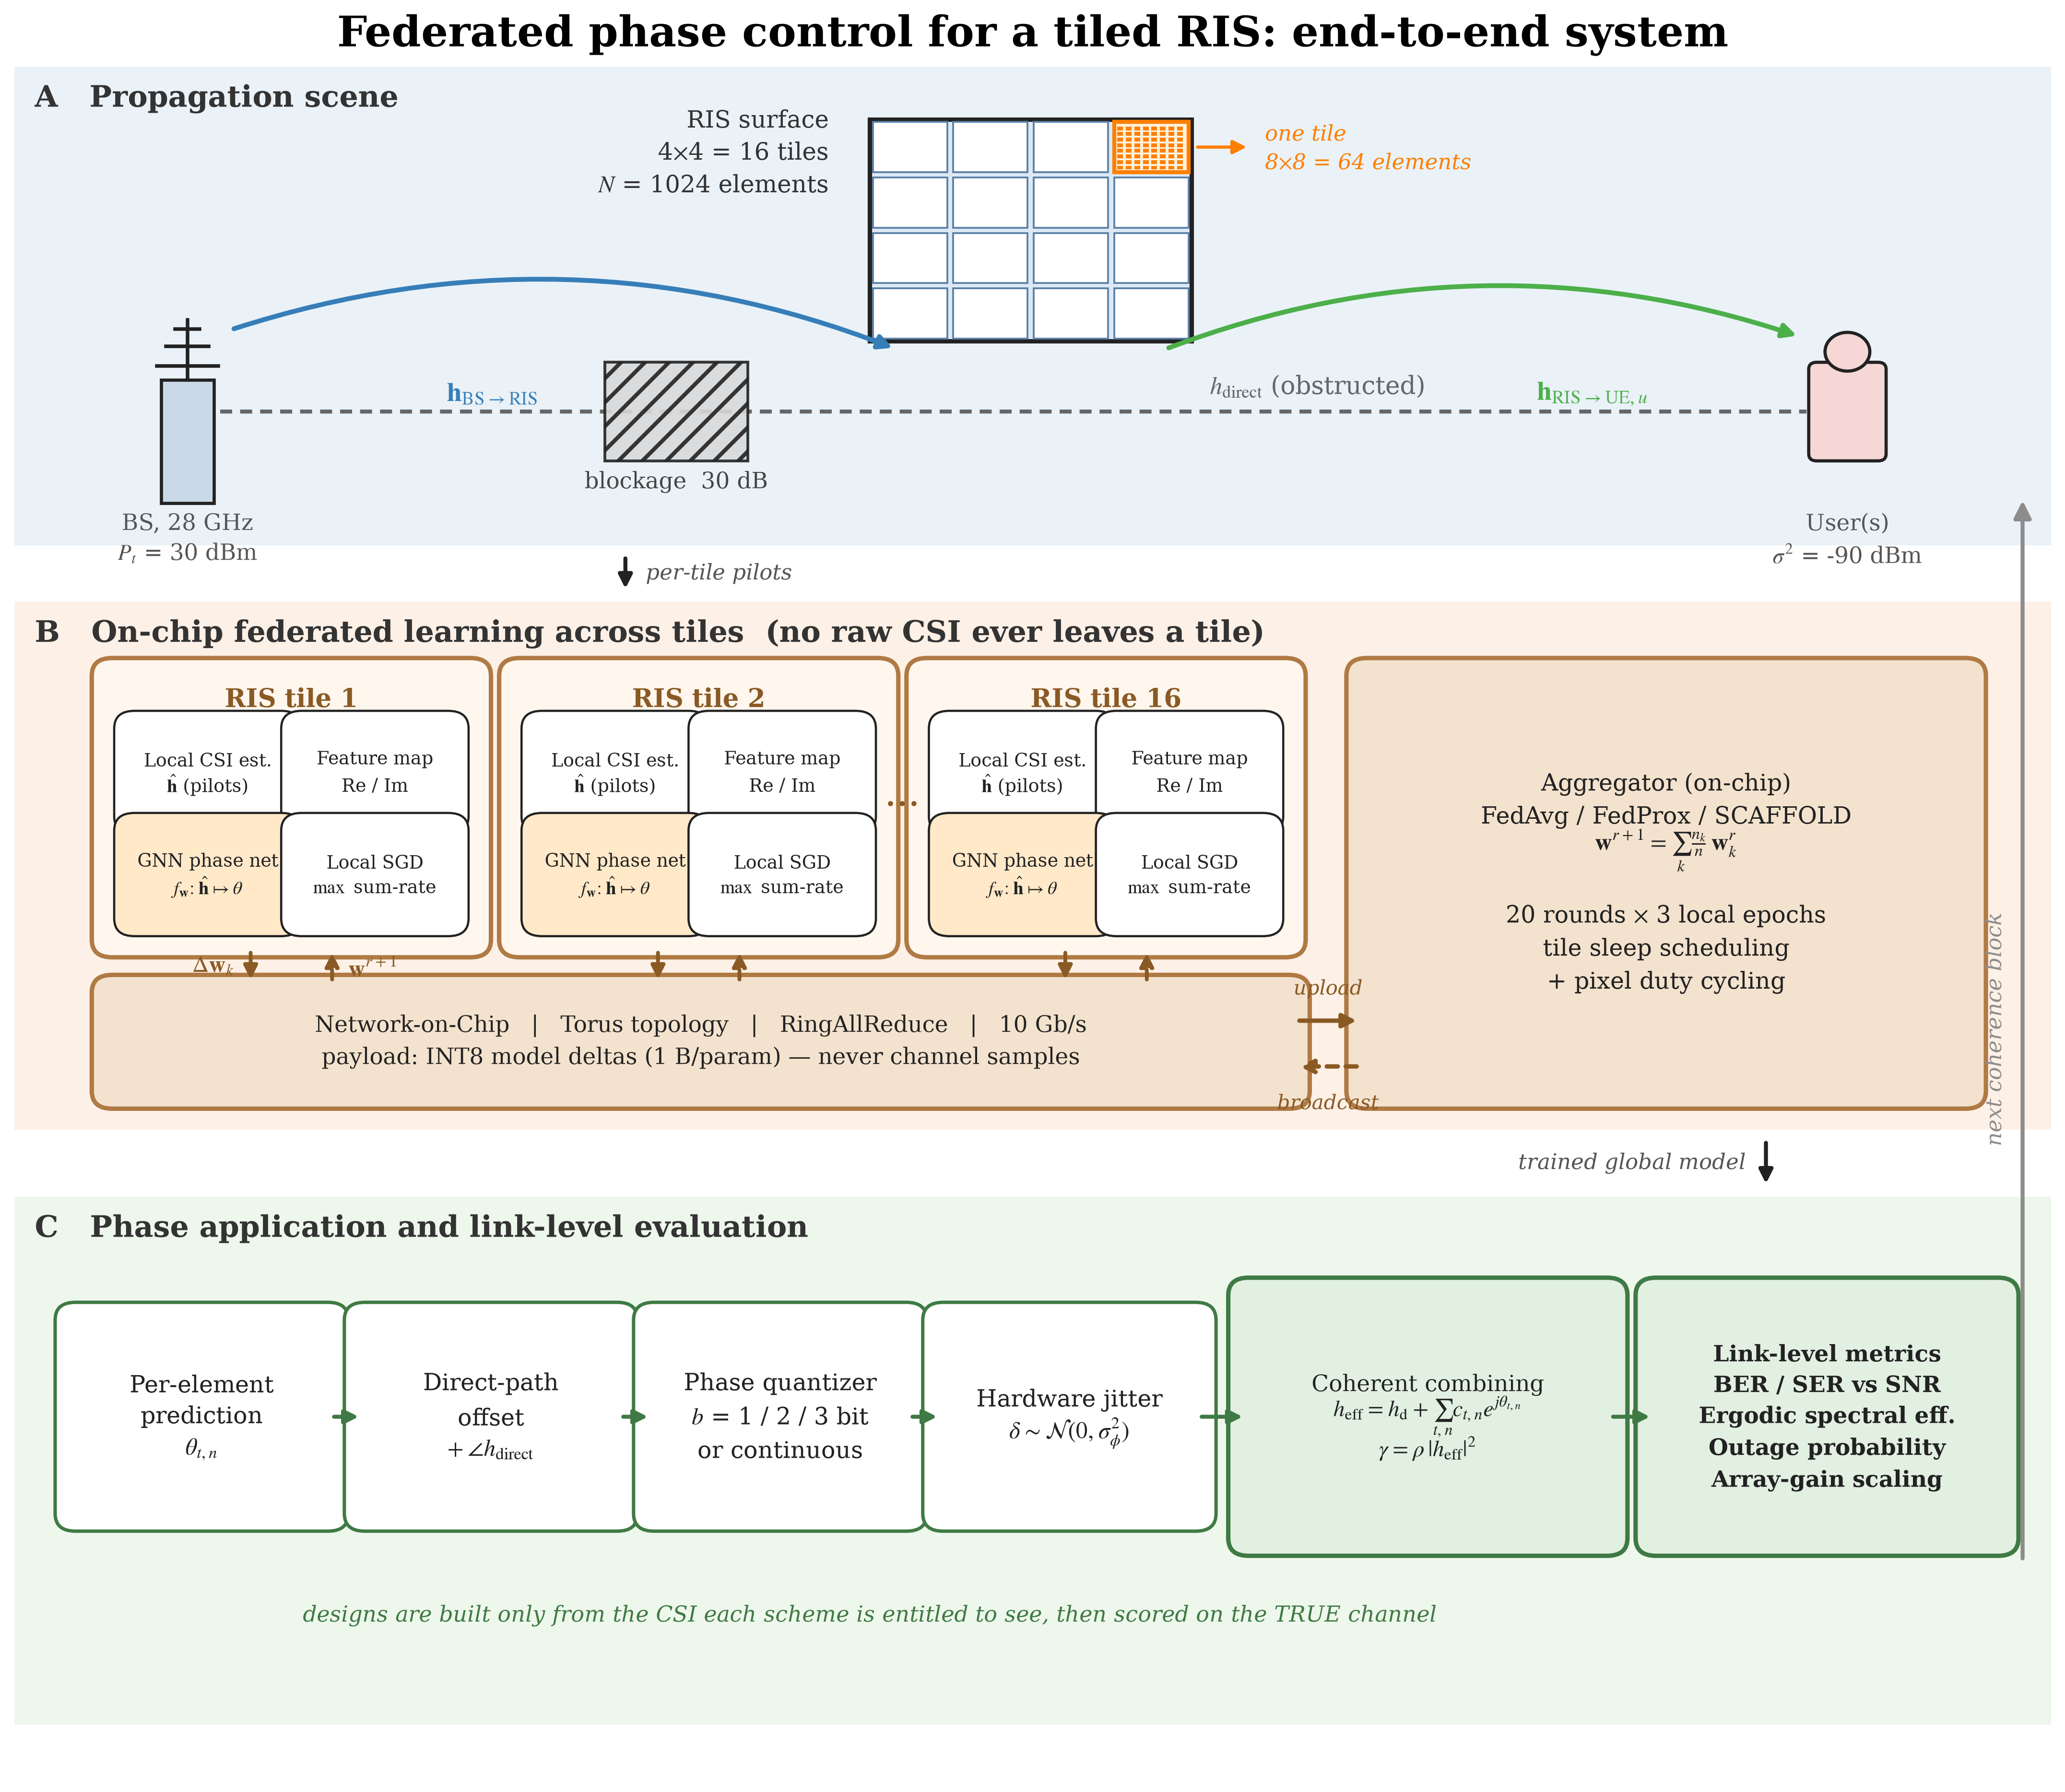
\includegraphics[width=\textwidth]{system_architecture.png}
\caption{End-to-end Fed-RIS architecture. (A)~Propagation scene with 28\,GHz blocked direct path and 1024-element tiled RIS. (B)~On-chip federated learning: each tile trains a local GAT phase net, INT8 deltas are aggregated via NoC. (C)~Phase application pipeline with quantization, jitter, and link-level evaluation.}
\label{fig:arch}
\end{figure*}

\subsection{Hardware Impairments}

Predicted phases undergo three hardware degradations before scoring:
\begin{itemize}
\item \textbf{$b$-bit uniform quantization}: $\theta_q = \text{round}(\theta / \Delta) \cdot \Delta$, where $\Delta = 2\pi / 2^b$. The theoretical array-gain penalty is $20\log_{10}\text{sinc}(2^{-b})$~\cite{wu2020discrete}.
\item \textbf{Phase jitter}: $\theta_\text{applied} = \theta_q + \delta$, where $\delta \sim \mathcal{N}(0, \sigma_\phi^2)$.
\item \textbf{CSI estimation error}: $\hat{\bm{h}} = \bm{h} + \bm{e}$, where $\bm{e} \sim \mathcal{CN}(0, \epsilon \cdot \mathbb{E}[|\bm{h}|^2])$, using normalized error variance $\epsilon$.
\end{itemize}

%% ===================================================================
%% III. BASELINE SCHEMES
%% ===================================================================
\section{Baseline Comparison Framework}
\label{sec:baselines}

All schemes are scored on identical channel realizations (600 test scenes, seed 42). Each scheme designs its phases from the CSI it is entitled to access and is then evaluated against the true channel.

\begin{table}[t]
\centering
\caption{Operational Requirements of Compared Schemes}
\label{tab:requirements}
\renewcommand{\arraystretch}{1.1}
\setlength{\tabcolsep}{3pt}
\footnotesize
\begin{tabular}{@{}lcccc@{}}
\toprule
\textbf{Scheme} & \textbf{CSI Req.} & \textbf{Per-Block} & \textbf{Local} & \textbf{$O(\cdot)$} \\
\midrule
No RIS & --- & --- & \checkmark & $O(1)$ \\
Random & None & None & \checkmark & $O(N)$ \\
AO~\cite{wu2020joint} & Full & Iterative & $\times$ & $O(NI)$ \\
SCA~\cite{guo2020} & Full & Iterative & $\times$ & $O(NI)$ \\
Centralized DL & Pooled & 1 fwd & $\times$ & $O(N)$ \\
\textbf{Fed-RIS} & \textbf{Local} & \textbf{1 fwd} & \checkmark & $O(N)$ \\
MRC (bound) & Perfect & Closed & --- & $O(N)$ \\
\bottomrule
\end{tabular}
\end{table}

Table~\ref{tab:requirements} summarizes the operational requirements. Fed-RIS is unique in keeping CSI on-tile while achieving $O(N)$ single-forward-pass inference---no iterative solve per coherence block.

%% ===================================================================
%% IV. RESULTS
%% ===================================================================
\section{Experimental Results}
\label{sec:results}

Simulations use a 1024-element RIS (16 tiles $\times$ 64 elements), 28\,GHz carrier, 30\,dB blockage, Rician fading ($K\!=\!10$\,dB), 600 test scenes, 20 FL rounds $\times$ 3 local epochs, and FedAvg aggregation with INT8 deltas over Torus NoC.

\subsection{BER Performance}

Fig.~\ref{fig:ber} shows BER vs.\ transmit SNR $\rho$ for QPSK and 16-QAM modulations. Fed-RIS achieves BER\,$=10^{-3}$ at $\rho = 99.2$\,dB (QPSK), which is \textbf{36.7\,dB earlier} than the blocked direct link ($\rho = 135.9$\,dB) and only \textbf{1.3\,dB} behind the perfect-CSI MRC bound ($\rho = 97.9$\,dB). The gap to Centralized DL is a mere 1.1\,dB---the precise cost of keeping CSI distributed on-tile.

\begin{figure}[t]
\centering
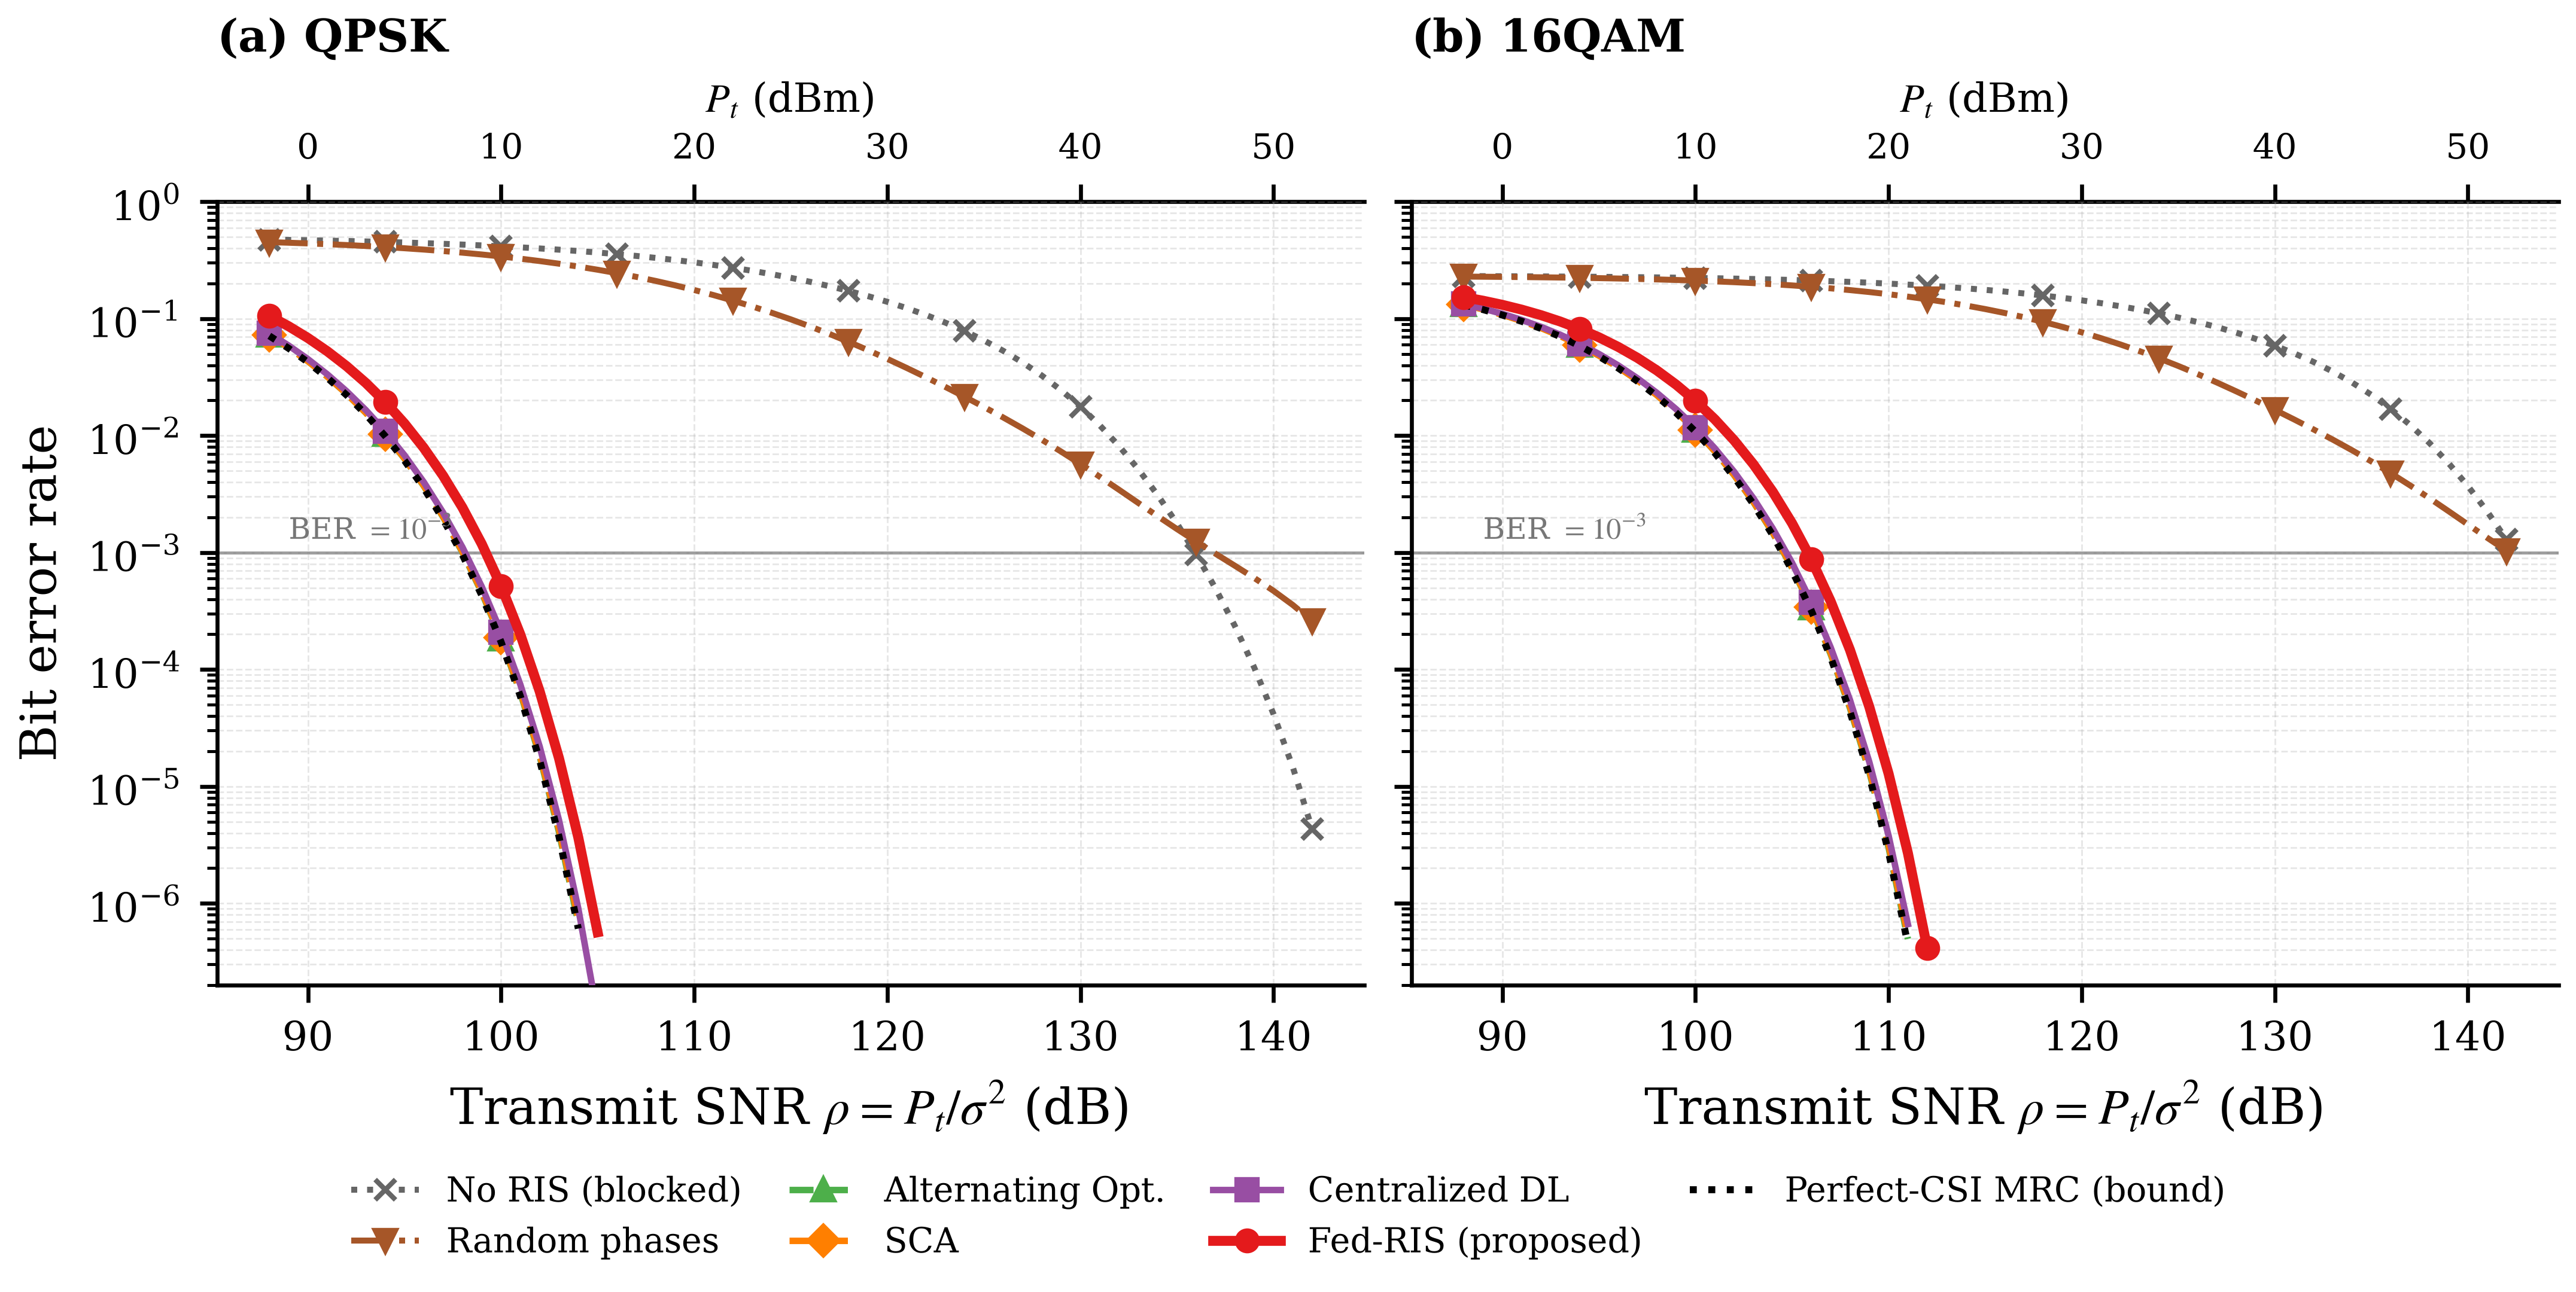
\includegraphics[width=\columnwidth]{fig1_ber_vs_snr.png}
\caption{BER vs.\ transmit SNR for QPSK (left) and 16-QAM (right). Fed-RIS closely tracks centralized optimization baselines and recovers 36.7\,dB of link budget over the blocked direct path.}
\label{fig:ber}
\end{figure}

\subsection{Spectral Efficiency and Power Savings}

Fig.~\ref{fig:se} presents the achievable spectral efficiency and transmit-power savings. At the operating point $\rho = 99$\,dB, Fed-RIS achieves 4.64\,bit/s/Hz compared to 0.16\,bit/s/Hz without RIS. The power-saving analysis at a target rate of 4\,bit/s/Hz shows that Fed-RIS provides a 31.4\,dB transmit-power reduction, within 1.9\,dB of the oracle MRC bound (33.3\,dB).

\begin{figure}[t]
\centering
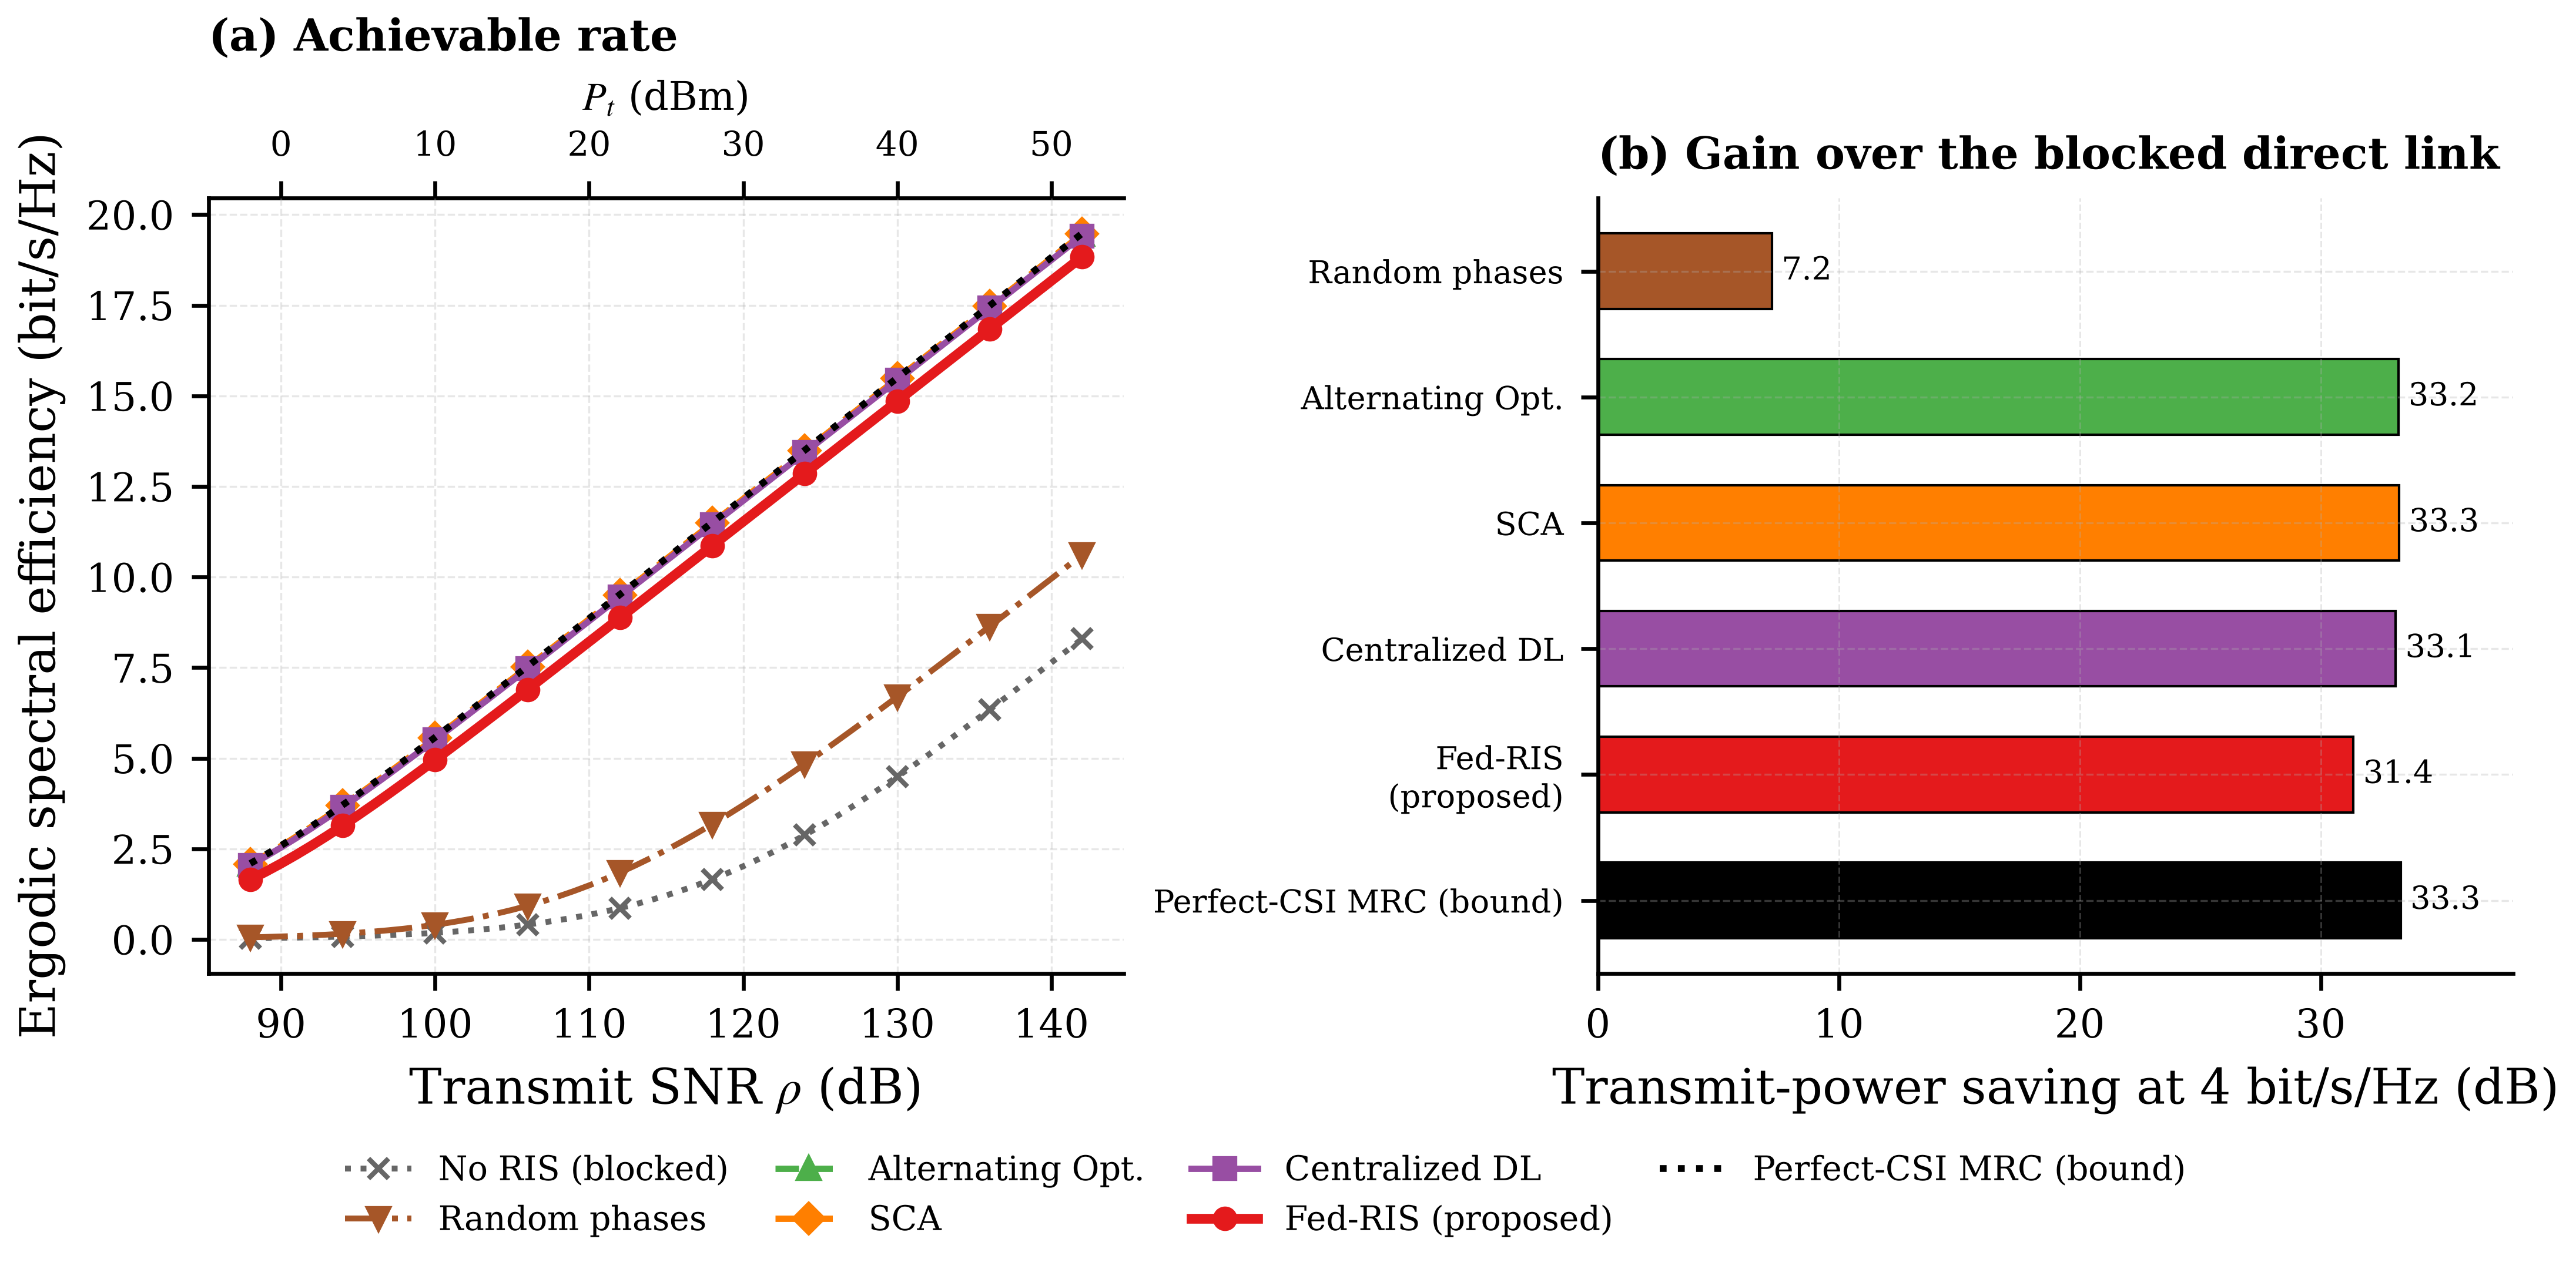
\includegraphics[width=\columnwidth]{fig2_spectral_efficiency.png}
\caption{(a) Achievable rate vs.\ SNR. (b) Transmit-power saving at 4\,bit/s/Hz target. Fed-RIS achieves 31.4\,dB power saving, only 1.9\,dB from the oracle bound.}
\label{fig:se}
\end{figure}

\subsection{Outage Probability}

Fig.~\ref{fig:outage} shows outage probability at rate thresholds $R_\text{th}=1$ and 2\,bit/s/Hz. Fed-RIS closely tracks the centralized baselines across all SNR values, providing a diversity gain that eliminates the deep outage floor present for the blocked direct link and random phases.

\begin{figure}[t]
\centering
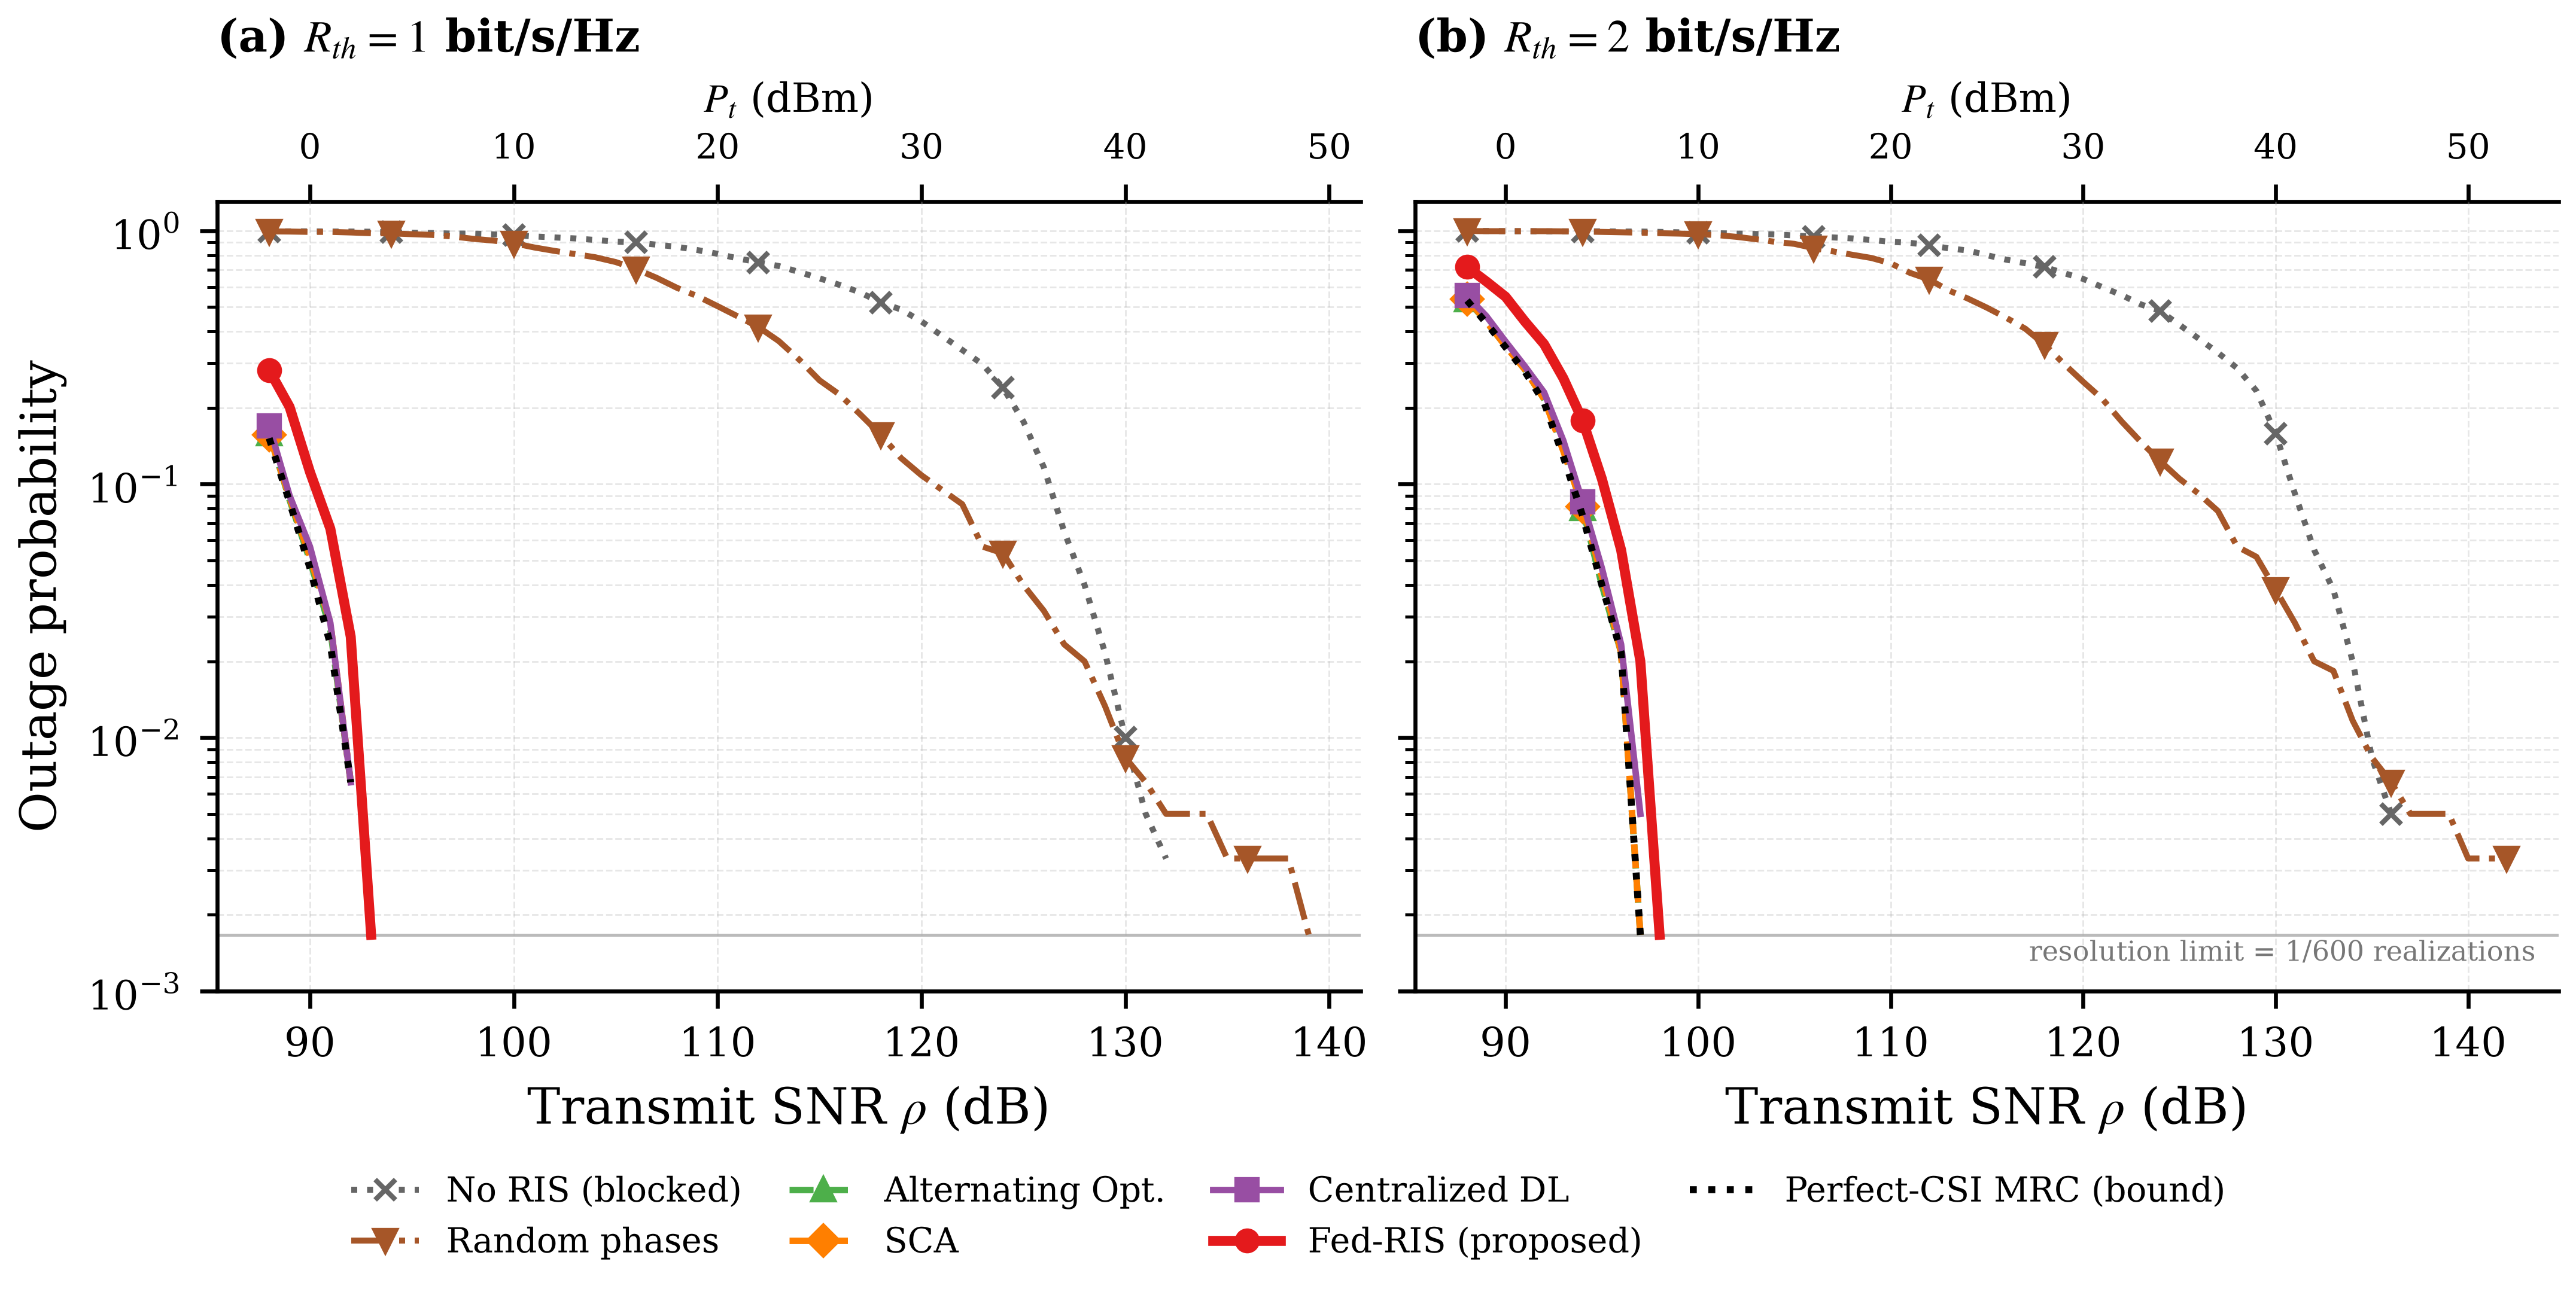
\includegraphics[width=\columnwidth]{fig3_outage_probability.png}
\caption{Outage probability at $R_\text{th}=1$ and 2\,bit/s/Hz. Fed-RIS closely tracks centralized optimization baselines.}
\label{fig:outage}
\end{figure}

\subsection{Hardware Impairments}

Fig.~\ref{fig:hw} presents the impact of phase quantization and jitter. Table~\ref{tab:quant} compares measured quantization losses against the theoretical $20\log_{10}\text{sinc}(2^{-b})$ bound. The 2-bit operating point incurs only ${\sim}0.82$\,dB loss for Fed-RIS, confirming practical deployability with low-cost phase shifters. Phase jitter is second-order: 5$^\circ$ RMS jitter causes only 0.03\,dB loss.

\begin{figure}[t]
\centering
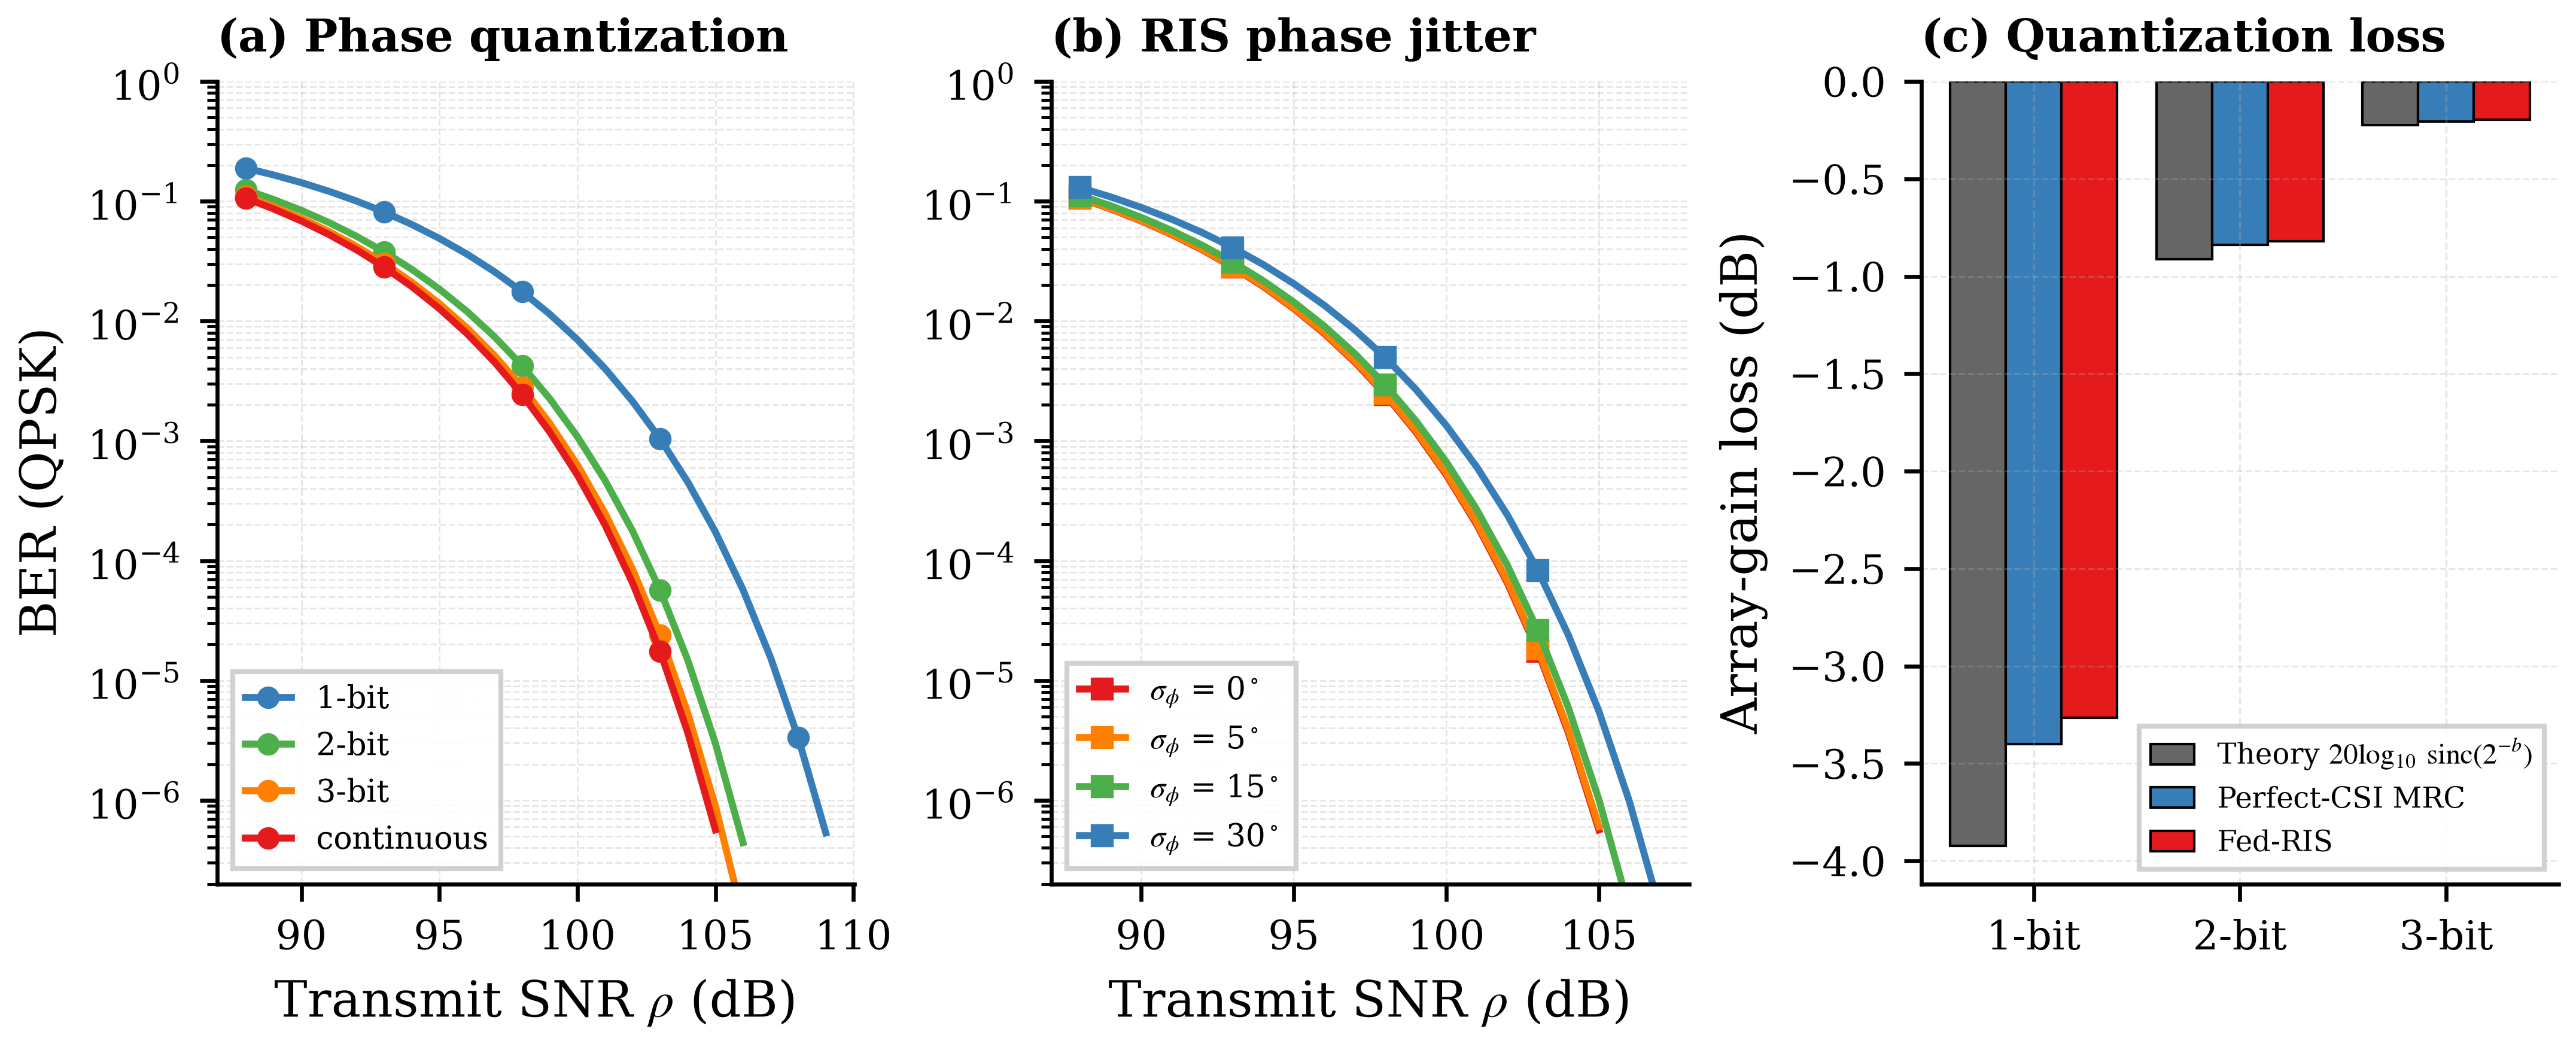
\includegraphics[width=\columnwidth]{fig4_hardware_impairments.png}
\caption{(a) BER under $b$-bit phase quantization. (b) BER under RMS phase jitter. (c) Measured quantization loss vs.\ theoretical sinc bound for Fed-RIS, MRC, and theory.}
\label{fig:hw}
\end{figure}

\begin{table}[t]
\centering
\caption{Phase Quantization Array-Gain Loss (dB)}
\label{tab:quant}
\renewcommand{\arraystretch}{1.1}
\footnotesize
\begin{tabular}{@{}lccc@{}}
\toprule
\textbf{Resolution} & \textbf{Theory} & \textbf{MRC} & \textbf{Fed-RIS} \\
\midrule
1-bit & $-3.92$ & $-3.40$ & $-3.26$ \\
2-bit & $-0.91$ & $-0.84$ & $-0.82$ \\
3-bit & $-0.22$ & $-0.21$ & $-0.20$ \\
Continuous & $0.00$ & $0.00$ & $0.00$ \\
\bottomrule
\end{tabular}
\end{table}

\subsection{CSI Robustness}

Fig.~\ref{fig:csi} reveals a key advantage of learned phase prediction: robustness under imperfect CSI. As normalized CSI error grows from $\epsilon\!=\!0$ to $\epsilon\!=\!1$, Fed-RIS loses only \textbf{3.2\,dB}, whereas model-based solvers (AO, SCA) degrade by \textbf{5.1\,dB}. Optimization-based methods treat flawed CSI as exact ground truth; the learned predictor incorporates implicit channel priors that provide graceful degradation. Notably, at $\epsilon\!=\!1$ all intelligent schemes converge to similar performance.

\begin{figure}[t]
\centering
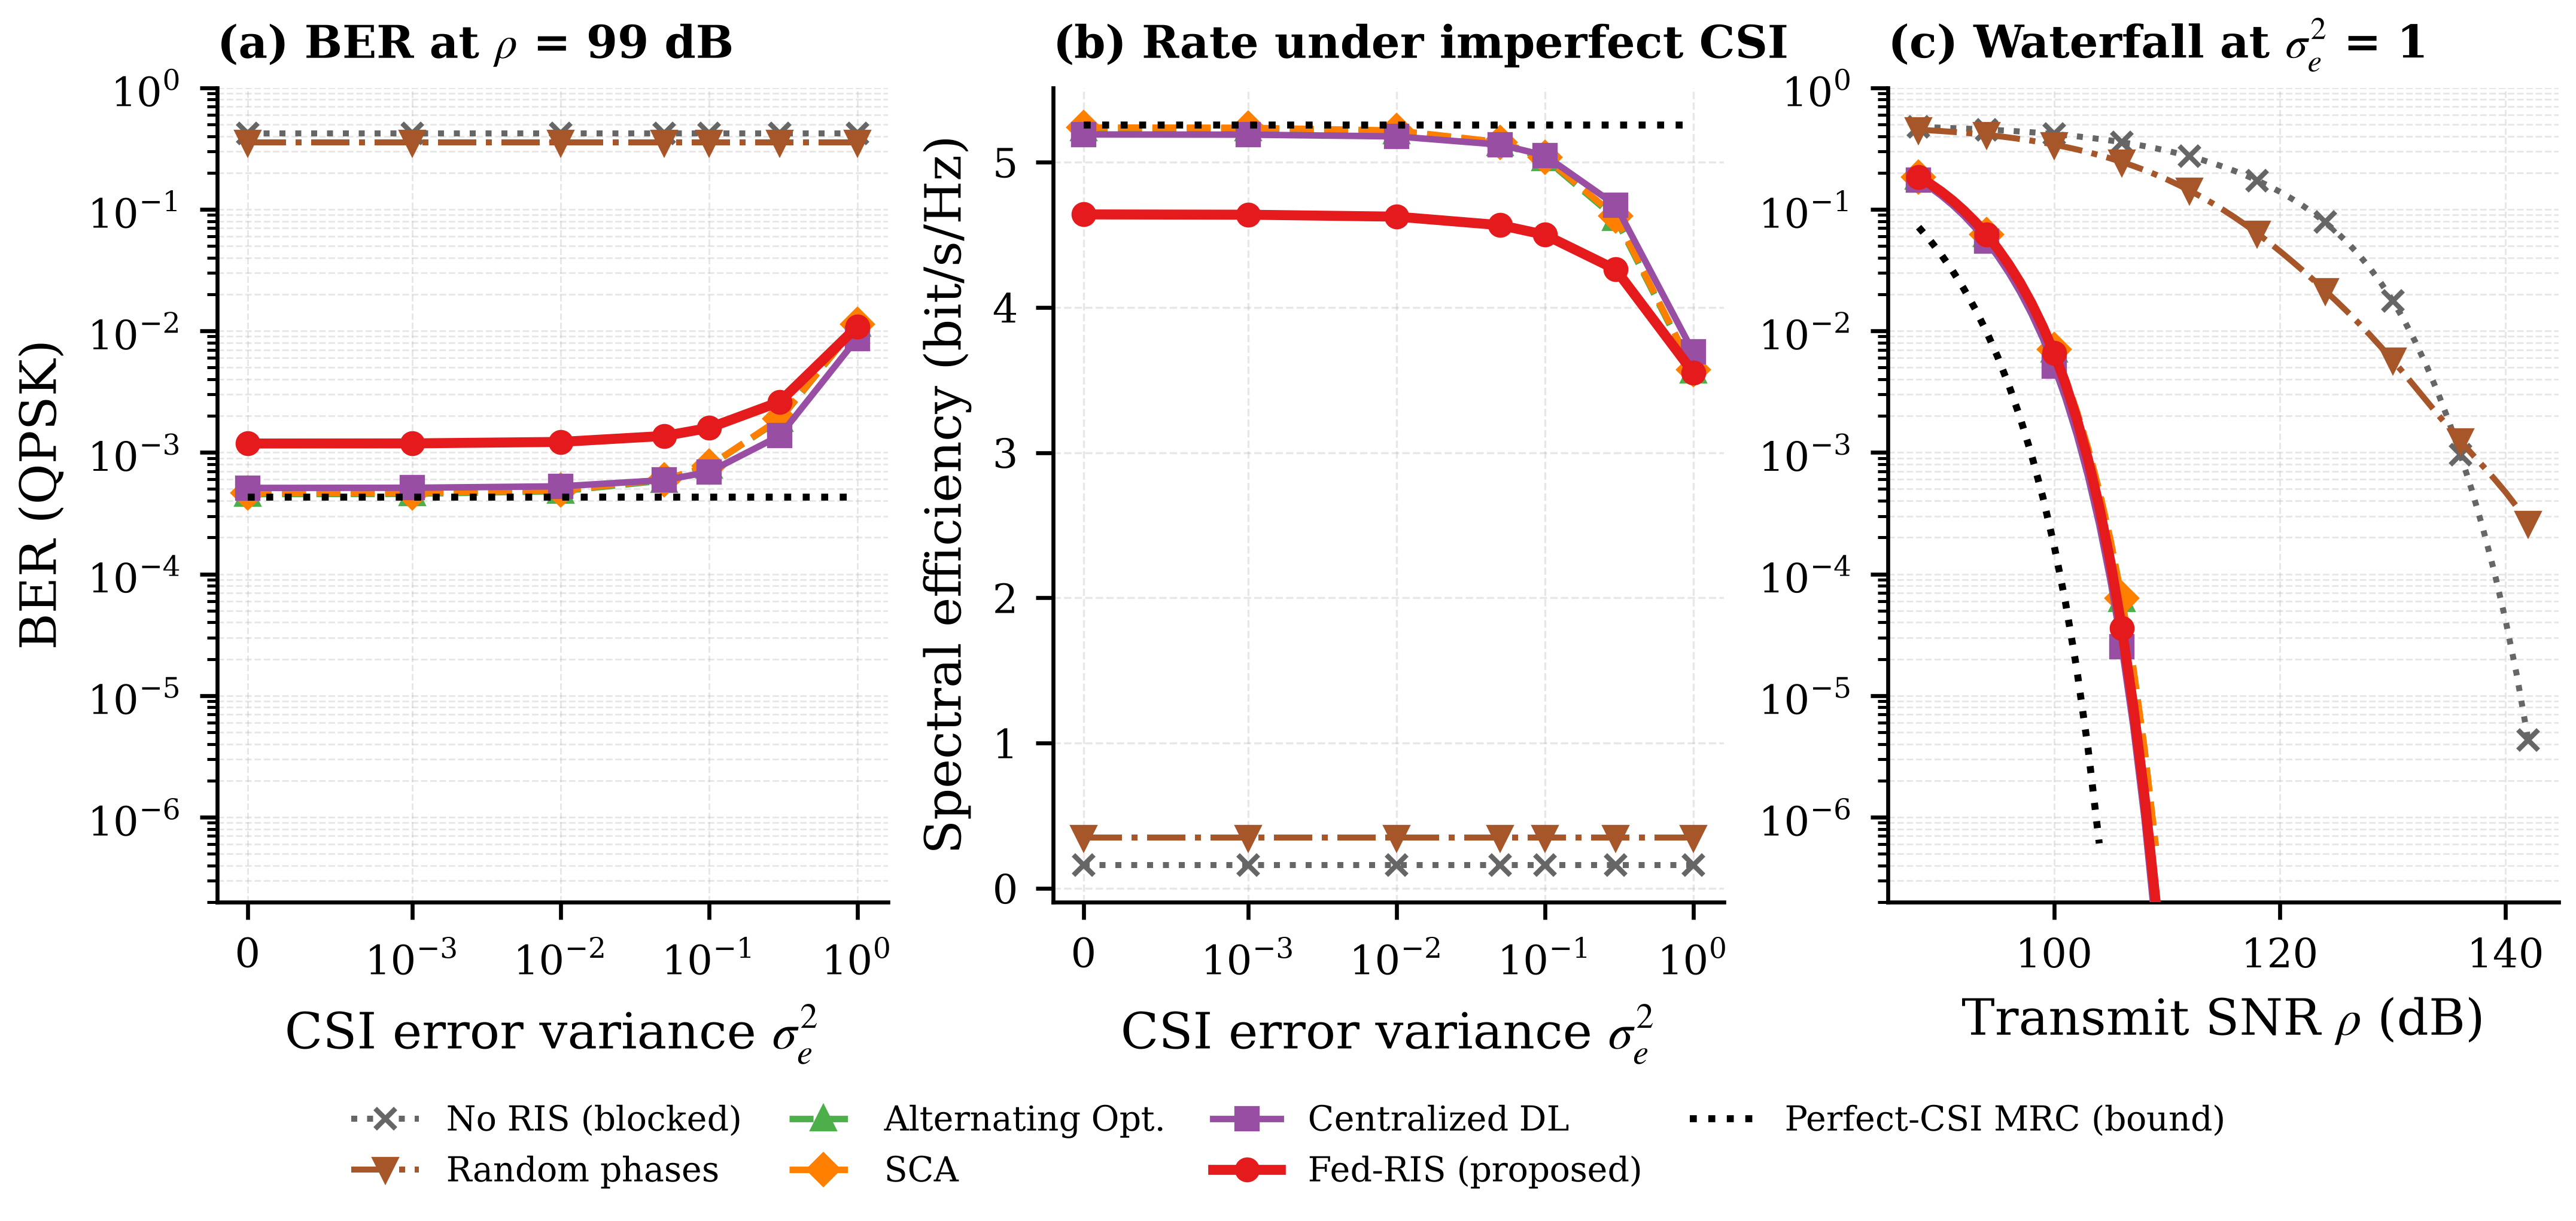
\includegraphics[width=\columnwidth]{fig5_csi_robustness.png}
\caption{CSI robustness comparison. (a) BER at $\rho\!=\!99$\,dB vs.\ CSI error. (b) Spectral efficiency vs.\ CSI error. (c) BER waterfall at $\epsilon\!=\!1$. Fed-RIS loses only 3.2\,dB (vs.\ 5.1\,dB for AO/SCA).}
\label{fig:csi}
\end{figure}

\subsection{Array-Gain Scaling}

Fig.~\ref{fig:scaling} validates the coherent combining $N^2$ scaling law. All intelligent schemes track $20\log_{10}N$ up to $N\!\approx\!512$, after which geometric path-loss from peripheral tiles causes saturation---a placement insight enabled by whole-surface modeling.

\begin{figure}[t]
\centering
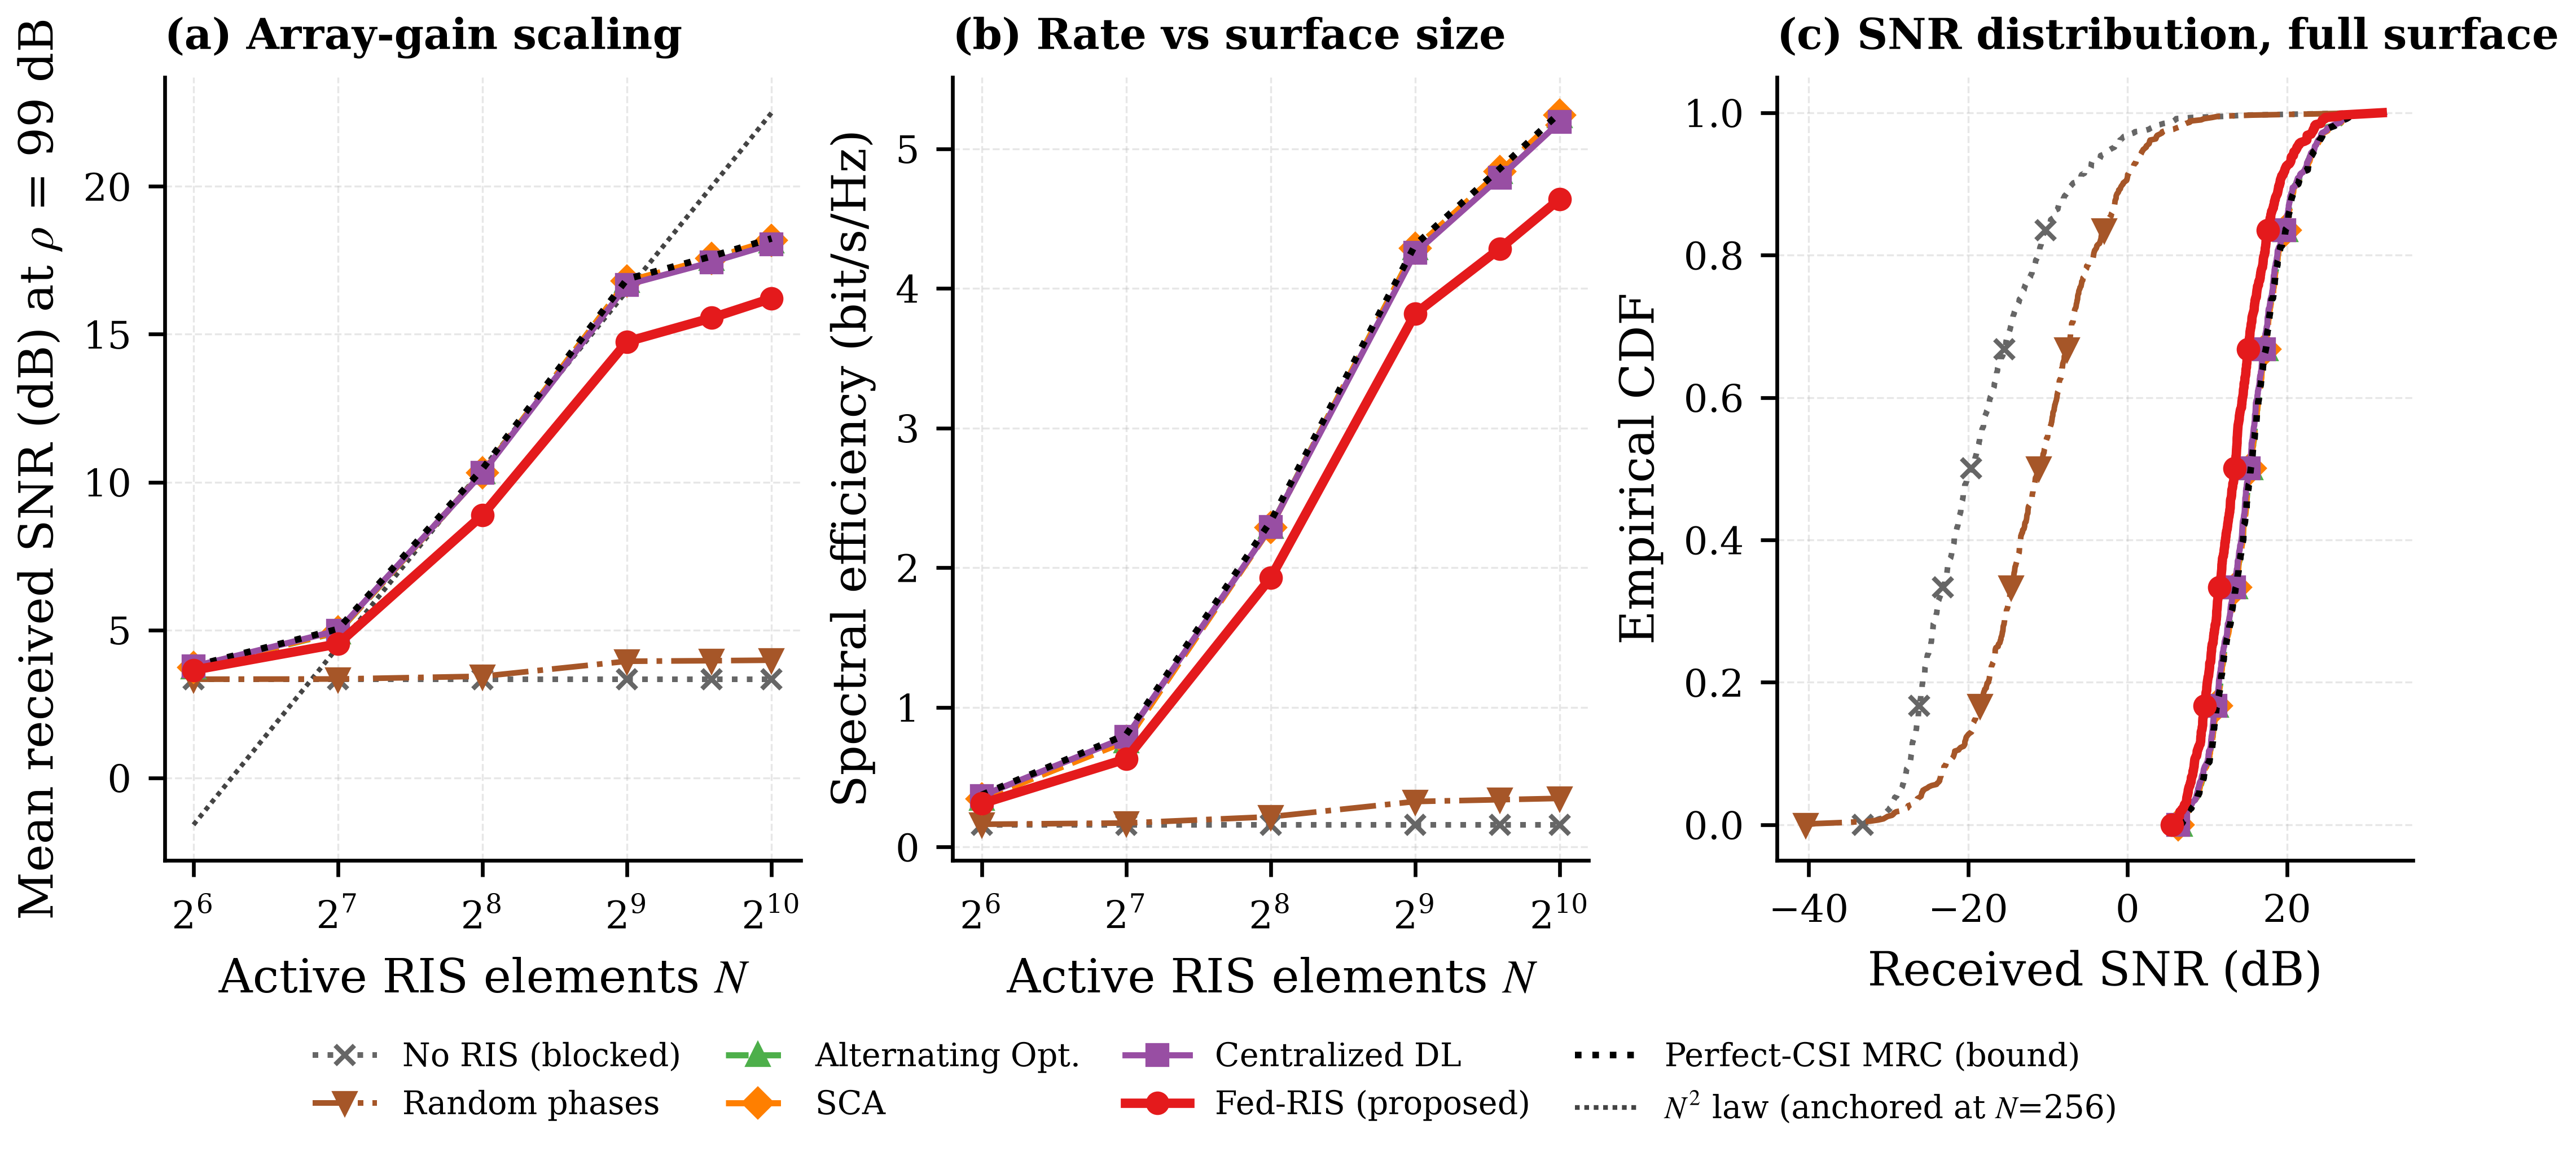
\includegraphics[width=\columnwidth]{fig6_array_scaling.png}
\caption{(a) Array-gain scaling with active elements $N$. (b) Spectral efficiency vs.\ $N$. (c) Received SNR distribution at full aperture. Coherent gain saturates beyond $N\!=\!512$ due to geometric path loss from peripheral tiles.}
\label{fig:scaling}
\end{figure}

\subsection{Communication Cost Analysis}

Table~\ref{tab:cost} presents the honest cost accounting. At 316K parameters and 600 training samples/tile, FL moves 39.6$\times$ more bytes (192.8\,MB in INT8 deltas) than centralized raw-CSI upload (4.9\,MB). FL becomes bandwidth-cheaper only above ${\sim}23{,}752$ samples/tile. The honest claim for Fed-RIS is therefore \textbf{CSI privacy/locality} and \textbf{$O(N)$ inference latency}, not communication savings at this scale.

\begin{table}[t]
\centering
\caption{Training and Per-Coherence-Block Cost}
\label{tab:cost}
\renewcommand{\arraystretch}{1.1}
\footnotesize
\begin{tabular}{@{}lr@{}}
\toprule
\textbf{Metric} & \textbf{Value} \\
\midrule
Model parameters & 315,906 \\
FL rounds $\times$ local epochs & $20 \times 3$ \\
Total NoC traffic (INT8) & 192.8\,MB \\
Raw-CSI upload (centralized) & 4.9\,MB \\
Traffic ratio (FL / raw CSI) & 39.6$\times$ \\
FL-cheaper crossover & ${\sim}$23,752 samples/tile \\
Per-block solve: AO & 21.9\,ms \\
Per-block solve: SCA & 2.0\,ms \\
Per-block inference: Fed-RIS & 1 fwd pass \\
\bottomrule
\end{tabular}
\end{table}

%% ===================================================================
%% V. DISCUSSION
%% ===================================================================
\section{Discussion}

\textbf{Novelty and positioning.} Existing federated approaches for wireless treat user devices~\cite{mcmahan2017} or base stations as clients with independent outputs. In Fed-RIS, the clients are metasurface tiles whose outputs are \emph{physically summed}---per-tile loss is meaningless without aperture-level coherent summation. This creates a fundamentally different FL problem where the network links are on-chip interconnects with physical topology and energy constraints~\cite{dally2004, bjerregaard2006}, and non-IID data arises from spatial geometry rather than synthetic partitioning.

\textbf{Honest limitations.} (i) With perfect CSI ($\epsilon\!=\!0$), closed-form MRC is provably optimal; Fed-RIS trails by 1.3\,dB. The case for Fed-RIS is on the cost axis (CSI locality, $O(N)$ inference) and the robustness axis ($\epsilon > 0$). (ii) The base evaluation uses a single-antenna BS and single dominant user. (iii) Channels are synthetic Rician/3GPP-UMi; DeepMIMO ray-tracing integration exists but was not used for reported runs.

%% ===================================================================
%% VI. CONCLUSION
%% ===================================================================
\section{Conclusion}

We presented Fed-RIS, a framework that federates phase optimization across the tiles of a single reconfigurable intelligent surface using on-chip learning over a Network-on-Chip. On 1024-element 28\,GHz mmWave channels with 30\,dB blockage, Fed-RIS recovers 36.7\,dB of link budget over the blocked direct path and sits within 1.3\,dB of the perfect-CSI MRC oracle bound. Its learned phase predictor exhibits superior robustness under imperfect CSI (3.2\,dB loss vs.\ 5.1\,dB for model-based solvers at $\epsilon\!=\!1$), and hardware non-idealities (2-bit quantization, $5^\circ$ jitter) cause negligible additional loss. The framework maintains full CSI privacy---raw channel measurements never leave the tile---while enabling constant-time $O(N)$ inference without per-coherence-block iterative optimization.

%% ===================================================================
%% REFERENCES
%% ===================================================================
\begin{thebibliography}{20}

\bibitem{wu2020joint}
Q.~Wu and R.~Zhang, ``Intelligent reflecting surface enhanced wireless network via joint active and passive beamforming,'' \emph{IEEE Trans. Wireless Commun.}, vol.~19, no.~8, pp.~5247--5261, Aug. 2020.

\bibitem{wu2020discrete}
Q.~Wu and R.~Zhang, ``Beamforming optimization for wireless network aided by intelligent reflecting surface with discrete phase shifts,'' \emph{IEEE Trans. Wireless Commun.}, vol.~19, no.~4, pp.~1838--1852, Apr. 2020.

\bibitem{direnzo2020}
M.~Di~Renzo \emph{et~al.}, ``Smart radio environments empowered by reconfigurable intelligent surfaces: How it works, state of research, and the road ahead,'' \emph{IEEE J. Sel. Areas Commun.}, vol.~38, no.~11, pp.~2450--2525, Nov. 2020.

\bibitem{rappaport2019}
T.~S.~Rappaport \emph{et~al.}, ``Wireless communications and applications above 100~GHz: Opportunities and challenges for 6G and beyond,'' \emph{IEEE Access}, vol.~7, pp.~78729--78757, 2019.

\bibitem{guo2020}
H.~Guo, Y.-C.~Liang, J.~Chen, and E.~G.~Larsson, ``Weighted sum-rate maximization for reconfigurable intelligent surface aided wireless networks,'' \emph{IEEE Trans. Wireless Commun.}, vol.~19, no.~5, pp.~3064--3076, May 2020.

\bibitem{yu2020admm}
S.~Yu, X.~Liu, and C.~Zhong, ``ADMM for intelligent reflecting surface-enhanced wireless networks,'' \emph{IEEE J. Sel. Areas Commun.}, vol.~38, no.~11, pp.~2550--2562, Nov. 2020.

\bibitem{luo2010}
Z.-Q.~Luo, W.-K.~Ma, A.~M.-C.~So, Y.~Ye, and S.~Zhang, ``Semidefinite relaxation of quadratic optimization problems,'' \emph{IEEE Signal Process. Mag.}, vol.~27, no.~3, pp.~20--34, May 2010.

\bibitem{huang2020drl}
C.~Huang \emph{et~al.}, ``Reconfigurable intelligent surface assisted multi-user MISO systems exploiting deep reinforcement learning,'' \emph{IEEE J. Sel. Areas Commun.}, vol.~38, no.~8, pp.~1839--1850, Aug. 2020.

\bibitem{mcmahan2017}
B.~McMahan, E.~Moore, D.~Ramage, S.~Hampson, and B.~A.~y~Arcas, ``Communication-efficient learning of deep networks from decentralized data,'' in \emph{Proc. AISTATS}, 2017, pp.~1273--1282.

\bibitem{li2020fedprox}
T.~Li, A.~K.~Sahu, M.~Zaheer, M.~Sanjabi, A.~Talwalkar, and V.~Smith, ``Federated optimization in heterogeneous networks,'' in \emph{Proc. MLSys}, 2020.

\bibitem{karimireddy2020}
S.~P.~Karimireddy, S.~Kale, M.~Mohri, S.~Reddi, S.~Stich, and A.~T.~Suresh, ``SCAFFOLD: Stochastic controlled averaging for federated learning,'' in \emph{Proc. ICML}, 2020, pp.~5132--5143.

\bibitem{shen2021gnn}
Y.~Shen, Y.~Shi, J.~Zhang, and K.~B.~Letaief, ``Graph neural networks for scalable radio resource management: Architecture design and theoretical analysis,'' \emph{IEEE J. Sel. Areas Commun.}, vol.~39, no.~1, pp.~101--115, Jan. 2021.

\bibitem{he2022gat}
S.~He, S.~Xiong, Y.~Ou, J.~Zhang, J.~Wang, Y.~Huang, and Y.~Zhang, ``An overview on the application of graph neural networks in wireless networks,'' \emph{IEEE Open J. Commun. Soc.}, vol.~3, pp.~2067--2089, 2022.

\bibitem{dally2004}
W.~J.~Dally and B.~Towles, \emph{Principles and Practices of Interconnection Networks}. Morgan Kaufmann, 2004.

\bibitem{bjerregaard2006}
T.~Bjerregaard and S.~Mahadevan, ``A survey of research and practices of network-on-chip,'' \emph{ACM Comput. Surv.}, vol.~38, no.~1, pp.~1--51, 2006.

\bibitem{patarasuk2009}
P.~Patarasuk and X.~Yuan, ``Bandwidth optimal all-reduce algorithms for clusters of workstations,'' \emph{J. Parallel Distrib. Comput.}, vol.~69, no.~2, pp.~117--124, 2009.

\bibitem{sergeev2018}
A.~Sergeev and M.~Del~Balso, ``Horovod: Fast and easy distributed deep learning in TensorFlow,'' \emph{arXiv:1802.05799}, 2018.

\bibitem{zheng2022}
B.~Zheng, Q.~Wu, and R.~Zhang, ``Intelligent reflecting surface-aided mobile edge computing: Channel estimation and beamforming design,'' \emph{IEEE Trans. Wireless Commun.}, vol.~21, no.~6, pp.~4164--4179, Jun. 2022.

\bibitem{eisen2020}
M.~Eisen and A.~Ribeiro, ``Optimal wireless resource allocation with random edge graph neural networks,'' \emph{IEEE Trans. Signal Process.}, vol.~68, pp.~2977--2991, 2020.

\bibitem{huang2019}
C.~Huang, A.~Zappone, G.~C.~Alexandropoulos, M.~Debbah, and C.~Yuen, ``Reconfigurable intelligent surfaces for energy efficiency in wireless communication,'' \emph{IEEE Trans. Wireless Commun.}, vol.~18, no.~8, pp.~4157--4170, Aug. 2019.

\end{thebibliography}

\end{document}
